\documentclass[mathserif]{beamer}

\usepackage{parskip}
\usepackage{amsmath}
\usepackage{amssymb}
\usepackage{graphicx}

\frenchspacing

\logo{
\includegraphics[width=0.075\textwidth]{../Logo}}

\usetheme{Rochester}
\usecolortheme{whale}
%\beamertemplatenavigationsymbolsempty

\AtBeginSection[] {%
	\begin{frame}
		\frametitle{Table of Contents}
		\tableofcontents[currentsection]
	\end{frame}
}

\newenvironment{compactmath}[1][\normalsize]%
	{\begin{minipage}{\textwidth}\vspace{-0.75\baselineskip}#1\begin{equation*}}
	{\end{equation*}\end{minipage}}

\newenvironment{namedframe}[1]%
	{\begin{frame}\frametitle{#1}\framesubtitle{\secname}}
	{\end{frame}}


\usepackage{siunitx}
\usepackage{tikz}
\usepackage{tkz-euclide}
\usetkzobj{all}


\title{Geometry 1}
\author{Caroline Liu}
\date{
\includegraphics{../LicenseLogo}\\\copyright{} Caroline Liu, 2017}

\begin{document}
	\frame{\titlepage}
	\section{Introduction}
	\begin{namedframe}{Polygons}
		Polygons are 2D shapes that have 3 or more sides.
		\pause

		Polygons are named after the number of sides the shape has.
		\pause

		\begin{center}
			\begin{tabular}{|c|c|c|}
				\hline
				Sides & Prefix & Name\\\hline
				3     & Tri    & Triangle\\
				4     & Quad   & Quadrilateral\\
				5     & Penta  & Pentagon\\\hline
			\end{tabular}
		\end{center}
	\end{namedframe}
	\begin{namedframe}{Angles}
		The sum of a shape's interior angles can be found with this formula:
		\[\frac{180(n-2)}{n}\]
		\pause

		The sum of a shape's exterior angles can be found with this formula:
		\[360\si{\degree}\]
		(It's always \SI{360}{\degree}.)
		\pause

		These formulas are \alert{very} useful for contests.
	\end{namedframe}
	\begin{namedframe}{Shapes to look out for: without 3 sides}
		\begin{description}[<+->]
			\item[Trapezoids] Can often be split into 2 triangles and a rectangle. Questions include determining a dimension given other info, or calculating area. Very common contest question.
			\item[Parallelograms, squares, and rectangles] May be used in conjunction with circles, or you will be tasked with finding a dimension given some info. Also a common contest question.
		\end{description}
	\end{namedframe}
	\section{Triangles}
	\begin{namedframe}{Facts, formulas, and things to look out for}
		Triangles are one of the most common shapes found on contests. Whether it’s determining angles or sides, or deducing similar triangles, they are almost a guarantee. Basic concepts needed are the sum of the interior angles being \SI{180}{\degree}, and that the sum of 2 sides should never be larger than the 3rd side
		\pause

		Next, we'll go over some important concepts.
	\end{namedframe}
	\section{Pythagorean theorem}
	\begin{namedframe}{Your best friend}
		The Pythagorean theorem states that the relationship between the lengths of the sides of a right triangle is:
		\[a^2 + b^2 = c^2\]
		Where $a$ and $b$ are the legs of the triangle, and $c$ is the hypotenuse.

		\centering
		\begin{tikzpicture}
			\coordinate (A) at (4,4);
			\coordinate (B) at (0,0);
			\coordinate (C) at (4,0);

			\draw (A) -- (B) -- (C) -- cycle;

			\tkzLabelSegment[below=1pt](B,C){$a$};
			\tkzLabelSegment[right=1pt](A,C){$b$};
			\tkzLabelSegment[above left=1pt](A,B){$c$};
		\end{tikzpicture}
	\end{namedframe}
	\section{Important/special triangles}
	\begin{namedframe}{Pythagorean triplets}
		Pythagorean triplets are right triangles with three positive integer side lengths. A common example of this is a triangle whose side lengths have a ratio of $3:4:5$, or a multiple of that.

		Pythagorean triplets are a quick way to determine if certain triangles are a right triangle, and also useful for finding the side lengths of triangles.
	\end{namedframe}
	\begin{namedframe}{Pythagorean triplets example}
		\begin{columns}[c]
			\column{0.35\textwidth}
				\centering
				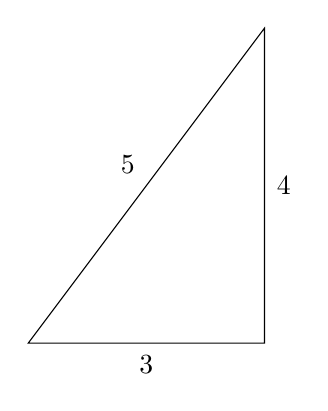
\begin{tikzpicture}
					\coordinate (A) at (0,0);
					\coordinate (B) at (3,0);
					\coordinate (C) at (3,4);

					\draw (A) -- (B) -- (C) -- cycle;

					\tkzLabelSegment[below=1pt](A,B){$3$};
					\tkzLabelSegment[above left=1pt](A,C){$5$};
					\tkzLabelSegment[right=1pt](B,C){$4$};
				\end{tikzpicture}
			\column{0.65\textwidth}
				\small
				\begin{proof}
					\vspace{-\baselineskip}
					\[a^2 + b^2 = c^2\]
					Let $LS$ be the left side of the equation: $a^2 + b^2$\\
					Let $RS$ be the right side of the equation: $c^2$

					Then $LS = RS$
					\begin{columns}[t]
						\column{0.5\textwidth}
							\begin{align*}
								LS &= a^2 + b^2\\
								LS &= 3^2 + 4^2\\
								LS &= 9 + 16\\
								LS &= 25
							\end{align*}
						\column{0.5\textwidth}
							\begin{align*}
								RS &= c^2\\
								RS &= 5^2\\
								RS &= 25
							\end{align*}
					\end{columns}
					\[LS = RS\qedhere\]
				\end{proof}
		\end{columns}
	\end{namedframe}
	\begin{namedframe}{\SI{30}{\degree}\thinspace--\thinspace\SI{60}{\degree}\thinspace--\thinspace\SI{90}{\degree} triangles}
		The ratio of the sides of a triangles with angles \SI{30}{\degree}, \SI{60}{\degree}, and \SI{90}{\degree} will always be $1:\sqrt{3}:2$.

		\centering
		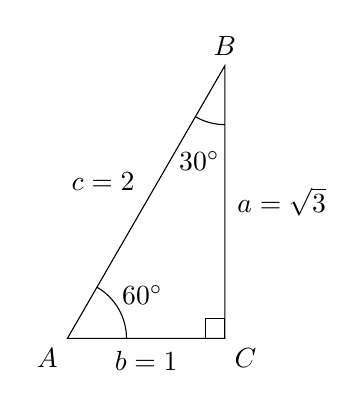
\begin{tikzpicture}
			\coordinate [label=below left:$A$] (A) at (0,0);
			\coordinate [label=above:$B$] (B) at (2,{2 * sqrt(3)});
			\coordinate [label=below right:$C$] (C) at (2,0);

			\draw (A) -- (B) -- (C) -- cycle;

			\tkzMarkAngle[size=0.75](C,A,B);
			\tkzLabelAngle[pos=1.1](C,A,B){$60\si{\degree}$};

			\tkzMarkAngle[size=0.75](A,B,C);
			\tkzLabelAngle[pos=1.25](A,B,C){$30\si{\degree}$};

			\tkzMarkRightAngle(A,C,B);

			\tkzLabelSegment[below=1pt](A,C){$b = 1$};
			\tkzLabelSegment[right=1pt](B,C){$a = \sqrt{3}$};
			\tkzLabelSegment[above left=1pt](A,B){$c = 2$};
		\end{tikzpicture}
	\end{namedframe}
	\begin{namedframe}{\SI{45}{\degree}\thinspace--\thinspace\SI{45}{\degree}\thinspace--\thinspace\SI{90}{\degree} triangles}
		The ratio of the sides of a triangles with angles \SI{45}{\degree}, \SI{45}{\degree}, and \SI{90}{\degree} will always be $1:1:\sqrt{2}$.

		\centering
		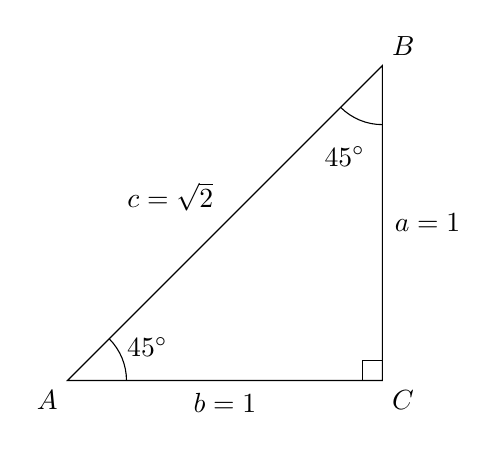
\begin{tikzpicture}
			\coordinate [label=below left:$A$] (A) at (0,0);
			\coordinate [label=above right:$B$] (B) at (4,4);
			\coordinate [label=below right:$C$] (C) at (4,0);

			\draw (A) -- (B) -- (C) -- cycle;

			\tkzMarkAngle[size=0.75](C,A,B);
			\tkzLabelAngle[pos=1.1](C,A,B){$45\si{\degree}$};

			\tkzMarkAngle[size=0.75](A,B,C);
			\tkzLabelAngle[pos=1.25](A,B,C){$45\si{\degree}$};

			\tkzMarkRightAngle(A,C,B);

			\tkzLabelSegment[below=1pt](A,C){$b = 1$};
			\tkzLabelSegment[right=1pt](B,C){$a = 1$};
			\tkzLabelSegment[above left=1pt](A,B){$c = \sqrt{2}$};
		\end{tikzpicture}
	\end{namedframe}
	\begin{namedframe}{Equilateral triangles}
		The ratio of the sides of a triangles with angles \SI{60}{\degree}, \SI{60}{\degree}, and \SI{60}{\degree} will always be $1:1:1$.

		\begin{center}
			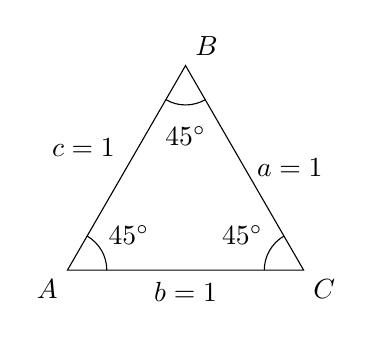
\begin{tikzpicture}
				\coordinate [label=below left:$A$] (A) at (0,0);
				\coordinate [label=above right:$B$] (B) at (1.5,{1.5 * sqrt(3)});
				\coordinate [label=below right:$C$] (C) at (3,0);

				\draw (A) -- (B) -- (C) -- cycle;

				\tkzMarkAngle[size=0.5](C,A,B);
				\tkzLabelAngle[pos=0.9](C,A,B){$45\si{\degree}$};

				\tkzMarkAngle[size=0.5](A,B,C);
				\tkzLabelAngle[pos=0.9](A,B,C){$45\si{\degree}$};

				\tkzMarkAngle[size=0.5](B,C,A);
				\tkzLabelAngle[pos=0.9](B,C,A){$45\si{\degree}$};

				\tkzLabelSegment[below=1pt](A,C){$b = 1$};
				\tkzLabelSegment[right=1pt](B,C){$a = 1$};
				\tkzLabelSegment[above left=1pt](A,B){$c = 1$};
			\end{tikzpicture}
		\end{center}
		\pause
		The area of an equilateral triangle with side length $s$ is:
		\[A = \frac{\sqrt{3} s^2}{4}\]
		We can prove this.
	\end{namedframe}
	\section{Trigonometric identities}
	\begin{namedframe}{SOHCAHTOA}
		\[\sin(\theta) = \frac{o}{h} \qquad \cos(\theta) = \frac{a}{h} \qquad \tan(\theta) = \frac{o}{a}\]
		\centering
		\begin{tikzpicture}
			\coordinate (A) at (0,0);
			\coordinate (B) at (4,4);
			\coordinate (C) at (4,0);

			\draw (A) -- (B) -- (C) -- cycle;

			\tkzMarkAngle[size=0.75](C,A,B);
			\tkzLabelAngle[pos=1.1](C,A,B){$\theta$};

			\tkzMarkRightAngle(A,C,B);

			\tkzLabelSegment[below=1pt](A,C){$a$};
			\tkzLabelSegment[right=1pt](B,C){$o$};
			\tkzLabelSegment[above left=1pt](A,B){$h$};
		\end{tikzpicture}
	\end{namedframe}
	\section{Similar triangles}
	\begin{namedframe}{What similar triangles are}
		Similar triangles have the same angles but different side lengths.

		\centering
		\begin{tikzpicture}
			\coordinate[label=below left:$A$](A) at (0,0);
			\coordinate[label=above:$B$](B) at (4,2);
			\coordinate[label=below right:$C$](C) at (6,0);

			\draw (A) -- (B) -- (C) -- cycle;
		\end{tikzpicture}
		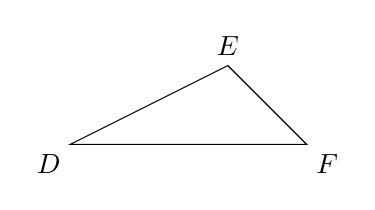
\begin{tikzpicture}
			\coordinate[label=below left:$D$](D) at (0,0);
			\coordinate[label=above:$E$](E) at (2,1);
			\coordinate[label=below right:$F$](F) at (3,0);

			\draw (D) -- (E) -- (F) -- cycle;
		\end{tikzpicture}
		\pause
		\[\triangle ABC \sim \triangle DEF\]
	\end{namedframe}
	\begin{namedframe}{Conditions for similarity}
		\begin{description}
			\item[Side, side, side (SSS)] If all 3 sides have the same ratio.
			\item[Angle, angle, angle (AAA)] If all 3 angles are the same.
			\item[Side, angle, side (SAS)] If 2 sides have the same ratio and 1 angle is the same.
		\end{description}
	\end{namedframe}
	\begin{namedframe}{SSS}
		\centering
		\begin{tikzpicture}
			\coordinate[label=below left:$A$](A) at (0,0);
			\coordinate[label=above:$B$](B) at (4,2);
			\coordinate[label=below right:$C$](C) at (6,0);

			\draw (A) -- (B) -- (C) -- cycle;
			\tkzLabelSegment[above left=1pt](A,B){$1$};
			\tkzLabelSegment[below=1pt](A,C){$2$};
			\tkzLabelSegment[above right=1pt](B,C){$3$};
		\end{tikzpicture}

		\vspace{1cm}

		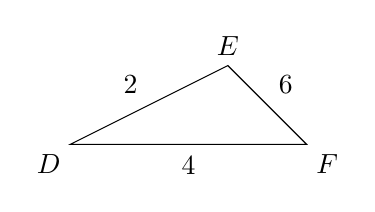
\begin{tikzpicture}
			\coordinate[label=below left:$D$](D) at (0,0);
			\coordinate[label=above:$E$](E) at (2,1);
			\coordinate[label=below right:$F$](F) at (3,0);

			\draw (D) -- (E) -- (F) -- cycle;

			\tkzLabelSegment[above left=1pt](D,E){$2$};
			\tkzLabelSegment[below=1pt](D,F){$4$};
			\tkzLabelSegment[above right=1pt](E,F){$6$};
		\end{tikzpicture}
	\end{namedframe}
	\begin{namedframe}{AAA}
		\centering
		\begin{tikzpicture}
			\coordinate[label=below left:$A$](A) at (0,0);
			\coordinate[label=above:$B$](B) at (4,3);
			\coordinate[label=below right:$C$](C) at (6,0);

			\draw (A) -- (B) -- (C) -- cycle;

			\tkzMarkAngle[size=0.75](C,A,B);
			\tkzLabelAngle[pos=1.1](C,A,B){$42\si{\degree}$};

			\tkzMarkAngle[size=0.75](A,B,C);
			\tkzLabelAngle[pos=1.1](A,B,C){$62\si{\degree}$};

			\tkzMarkAngle[size=0.75](B,C,A);
			\tkzLabelAngle[pos=1.1](B,C,A){$76\si{\degree}$};
		\end{tikzpicture}

		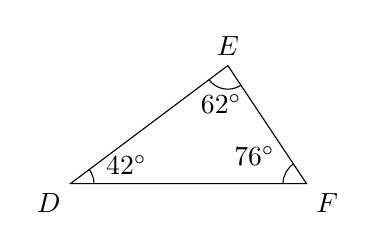
\begin{tikzpicture}
			\coordinate[label=below left:$D$](D) at (0,0);
			\coordinate[label=above:$E$](E) at (2,1.5);
			\coordinate[label=below right:$F$](F) at (3,0);

			\draw (D) -- (E) -- (F) -- cycle;

			\tkzMarkAngle[size=0.3](F,D,E);
			\tkzLabelAngle[pos=0.75](F,D,E){$42\si{\degree}$};

			\tkzMarkAngle[size=0.3](D,E,F);
			\tkzLabelAngle[pos=0.5](D,E,F){$62\si{\degree}$};

			\tkzMarkAngle[size=0.3](E,F,D);
			\tkzLabelAngle[pos=0.75](E,F,D){$76\si{\degree}$};
		\end{tikzpicture}
	\end{namedframe}
	\begin{namedframe}{SAS}
		\centering
		\begin{tikzpicture}
			\coordinate[label=below left:$A$](A) at (0,0);
			\coordinate[label=above:$B$](B) at (4,3);
			\coordinate[label=below right:$C$](C) at (6,0);

			\draw (A) -- (B) -- (C) -- cycle;

			\tkzMarkAngle[size=0.75](B,C,A);
			\tkzLabelAngle[pos=1.1](B,C,A){$76\si{\degree}$};

			\tkzLabelSegment[above left=1pt](A,B){$1$};
			\tkzLabelSegment[below=1pt](A,C){$2$};
		\end{tikzpicture}

		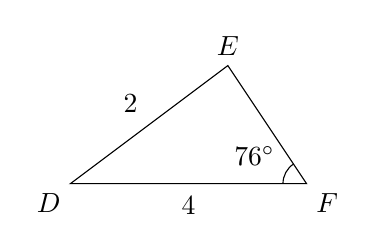
\begin{tikzpicture}
			\coordinate[label=below left:$D$](D) at (0,0);
			\coordinate[label=above:$E$](E) at (2,1.5);
			\coordinate[label=below right:$F$](F) at (3,0);

			\draw (D) -- (E) -- (F) -- cycle;

			\tkzMarkAngle[size=0.3](E,F,D);
			\tkzLabelAngle[pos=0.75](E,F,D){$76\si{\degree}$};

			\tkzLabelSegment[above left=1pt](D,E){$2$};
			\tkzLabelSegment[below=1pt](D,F){$4$};
		\end{tikzpicture}
	\end{namedframe}
	\section{Special lines }
	\begin{namedframe}{Bisectors/medians}
		Bisectors or medians are lines from a vertex to the middle of the opposite side.

		\centering
		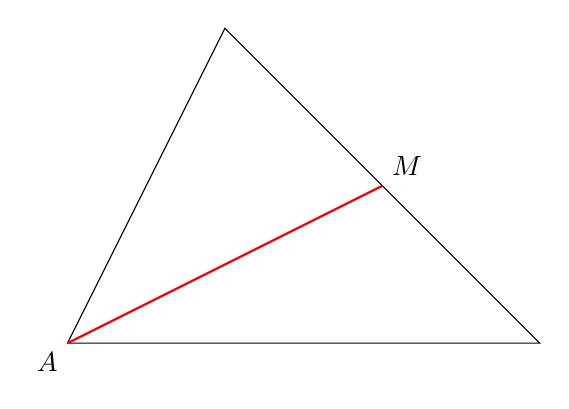
\begin{tikzpicture}
			\coordinate [label=below left:$A$] (A) at (0,0);
			\coordinate (B) at (6,0);
			\coordinate (C) at (2,4);
			\coordinate [label=above right:$M$] (M) at (4,2);

			\draw (A) -- (B) -- (C) -- cycle;
			\draw [red,thick] (A) -- (M);
		\end{tikzpicture}
	\end{namedframe}
	\begin{namedframe}{Angle bisectors}
		Angle bisectors are lines bisecting an angle.

		\centering
		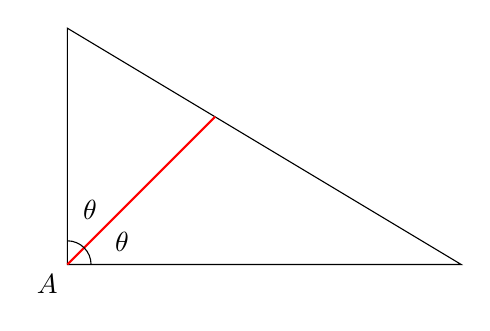
\begin{tikzpicture}
			\coordinate [label=below left:$A$] (A) at (0,0);
			\coordinate (B) at (5,0);
			\coordinate (C) at (0,3);
			\coordinate (M) at (1.875,1.875);

			\draw (A) -- (B) -- (C) -- cycle;
			\draw [red,thick] (A) -- (M);

			\tkzMarkAngle[fill=green,size=0.3](B,A,M);
			\tkzLabelAngle[pos=0.75](B,A,M){$\theta$};

			\tkzMarkAngle[fill=blue,size=0.3](M,A,C);
			\tkzLabelAngle[pos=0.75](M,A,C){$\theta$};
		\end{tikzpicture}
	\end{namedframe}
	\begin{namedframe}{Heights/altitudes}
		Heights or altitudes are lines perpendicular to a side that intersect the opposite vertex.

		\centering
		\begin{tikzpicture}
			\coordinate (A) at (0,0);
			\coordinate (B) at (5,0);
			\coordinate [label=above:$C$] (C) at (1,3);
			\coordinate [label=below:$M$] (M) at (1,0);

			\draw (A) -- (B) -- (C) -- cycle;

			\tkzMarkRightAngle(A,M,C);
			\tkzMarkRightAngle(B,M,C);

			\draw [red,thick] (M) -- (C);
		\end{tikzpicture}
	\end{namedframe}
	\begin{namedframe}{Perpendicular bisectors}
		Perpendicular bisectors are lines perpendicular to a side that also bisect it.

		\centering
		\begin{tikzpicture}
			\coordinate[label=below left:$A$](A) at (0,0);
			\coordinate[label=below right:$B$](B) at (5,0);
			\coordinate (C) at (1,3);
			\coordinate [label=below left:$M$](M) at (2.5,0);
			\coordinate (D) at (2.5,-3);
			\coordinate (E) at (2.5,3);

			\draw (A) -- (B) -- (C) -- cycle;

			\tkzMarkRightAngle(A,M,E);
			\tkzMarkRightAngle(B,M,D);

			\draw [red,thick] (D) -- (M) -- (E);
		\end{tikzpicture}
	\end{namedframe}
	\section{Special points of intersection}
	\begin{namedframe}{Orthocenter}
		The orthocenter is the point of intersection of the 3 altitudes of a triangle.

		\centering
		\begin{tikzpicture}[scale=0.5]
			\coordinate [label=left:$A$](A) at (-4,2);
			\coordinate [label=above:$B$](B) at (0,6);
			\coordinate [label=below left:$C$](C) at (6,-4);

			\coordinate [label=right:$O$](O) at (-3/2,7/2);

			\draw (A) -- (B) -- (C) -- cycle;

			\draw (A) -- (O);
			\draw (B) -- (O);
			\draw (C) -- (O);
		\end{tikzpicture}
	\end{namedframe}
	\begin{namedframe}{Centroid}
		The orthocenter is the point of intersection of the 3 medians of a triangle.
		\begin{center}
			\begin{tikzpicture}
				\coordinate [label=right:$A$](A) at (4,8);
				\coordinate [label=below:$B$](B) at (2,6);
				\coordinate [label=above left:$C$](C) at (0,10);

				\coordinate [label=above right:$M$](O) at (2,8);

				\draw (A) -- (B) -- (C) -- cycle;

				\draw (A) -- (O);
				\draw (B) -- (O);
				\draw (C) -- (O);
			\end{tikzpicture}
		\end{center}
		\pause
		The centroid splits each median into the ratio $2:1$.
	\end{namedframe}
	\begin{namedframe}{Incenter}
		The incenter is the point of intersection of the 3 angle bisectors of a triangle.
		\begin{center}
			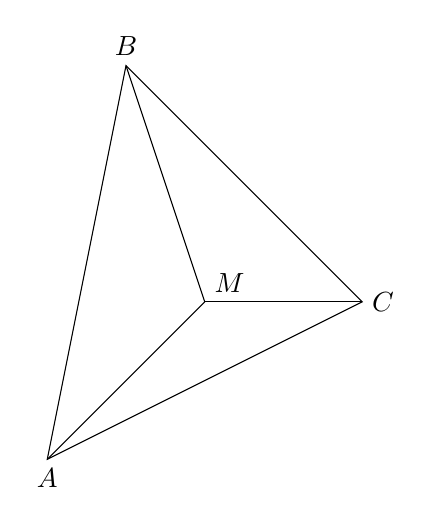
\begin{tikzpicture}
				\coordinate [label=below:$A$](A) at (1,1);
				\coordinate [label=above:$B$](B) at (2,6);
				\coordinate [label=right:$C$](C) at (5,3);

				\coordinate [label=above right:$M$](O) at (3,3);

				\draw (A) -- (B) -- (C) -- cycle;

				\draw (A) -- (O);
				\draw (B) -- (O);
				\draw (C) -- (O);
			\end{tikzpicture}
		\end{center}
		\pause
		The incenter is the centre of a triangle's incircle, the circle that has all points of the triangle on its circumference.
	\end{namedframe}
	\begin{namedframe}{Circumcenter}
		The circumcenter is the point of intersection of the 3 perpendicular bisectors of a triangle.
		\begin{center}
			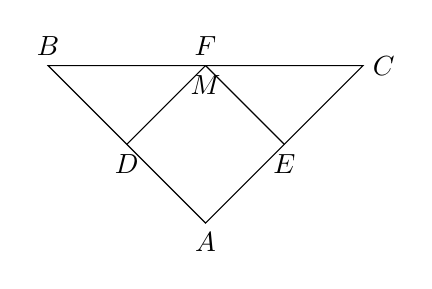
\begin{tikzpicture}
				\coordinate [label=below:$A$](A) at (3,2);
				\coordinate [label=above:$B$](B) at (1,4);
				\coordinate [label=right:$C$](C) at (5,4);

				\coordinate [label=below:$D$](D) at (2,3);
				\coordinate [label=below:$E$](E) at (4,3);
				\coordinate [label=above:$F$](F) at (3,4);

				\coordinate [label=below:$M$](O) at (3,4);

				\draw (A) -- (B) -- (C) -- cycle;

				\draw (D) -- (O);
				\draw (E) -- (O);
				\draw (F) -- (O);
			\end{tikzpicture}
		\end{center}
		\pause
		The circumcenter is the centre of triangle's incircle, the circle which is enclosed on all sides by the triangle. It is equidistant from all 3 sides of the triangle.
	\end{namedframe}
\end{document}
